
\subsection*{1.}

\begin{itemize}
    \item \( p(M) = \dfrac{1}{500} = \dfrac{2}{1000} = 0{,}002 \) ;
    \item \( p_M(S) = 0{,}95 \) ;
    \item \( p_{\overline{M}}(\overline{S}) = 0{,}96 \).
\end{itemize}

\subsection*{2.}

\begin{center}
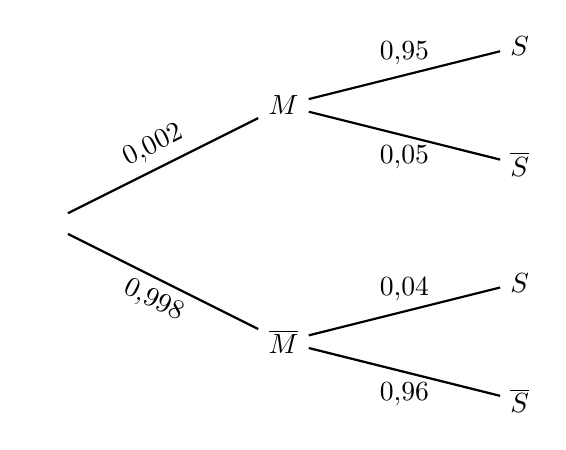
\begin{tikzpicture}[thick, scale=1.5]
\node (P_-1_0) at (-2,-1.5) {$\phantom{A}$};
\node (P_0_0) at (0,-0.5) {$M$};
\draw (P_-1_0) -- (P_0_0) node[midway, above,sloped] {$0{,}002$};
\node (P_1_0) at (2,-0) {$S$};
\draw (P_0_0) -- (P_1_0) node[midway, above] {$0{,}95$};
\node (P_1_1) at (2,-1) {$\overline{S}$};
\draw (P_0_0) -- (P_1_1) node[midway, below] {$0{,}05$};
\node (P_0_2) at (0,-2.5) {$\overline{M}$};
\draw (P_-1_0) -- (P_0_2) node[midway, below,sloped] {$0{,}998$};
\node (P_1_2) at (2,-2) {$S$};
\draw (P_0_2) -- (P_1_2) node[midway, above] {$0{,}04$};
\node (P_1_3) at (2,-3) {$\overline{S}$};
\draw (P_0_2) -- (P_1_3) node[midway, below] {$0{,}96$};
\end{tikzpicture}
\end{center}

\subsection*{3.}

On calcule :
\begin{itemize}
    \item \(p(M \cap S) = p(M) \times p_M(S) = 0{,}002 \times 0{,}95 = 0{,}0019,\)
    \item \(p(\overline{M} \cap S) = p(\overline{M}) \times p_{\overline{M}}(S) = 0{,}998 \times 0{,}04 = 0{,}03992\).
\end{itemize}
D'après la loi des probabilités totales :
\begin{align*}
p(S) &= p(M \cap S) + p(\overline{M} \cap S) \\
&= 0{,}0019 + 0{,}03992 \\
&= 0{,}04182.
\end{align*}

\subsection*{4.}

On a :
\[
p_S(M) = \dfrac{p(S \cap M)}{p(S)} = \dfrac{p(M \cap S)}{p(S)} = \dfrac{0{,}0019}{0{,}04182} \approx 0{,}0454,
\]
soit \(0{,}045\) au millième près (environ \(4{,}5 \, \% \)).

\subsection*{5.}

\begin{itemize}
    \item On a \( p(M \cap S) = 0{,}0019\) ;
    \item On a \( p(M) \times p(S) = 0{,}002 \times 0{,}04182 = 0{,}0008364\).
\end{itemize}
Donc \( p(M \cap S) \neq p(M) \times p(S) \) : les événements \( M \) et \( S \) ne sont pas indépendants.

